% Beamer slide template prepared by Tom Clark <tom.clark@op.ac.nz>
% Otago Polytechnic
% Dec 2012

\documentclass[10pt]{beamer}
\usetheme{CambridgeUS}
\usepackage{graphicx}
\usepackage{fancyvrb}
\usepackage{sidecap}


\title{Modelling Many-to-Many Relationships}

\author[IN705]{Databases Three}
\institute[Otago Polytechnic]{
  Otago Polytechnic \\
  Dunedin, New Zealand \\
}
\date{}
\begin{document}

%----------- titlepage ----------------------------------------------%
\begin{frame}[plain]
  \titlepage
\end{frame}



%----------- slide --------------------------------------------------%
\begin{frame}
  \frametitle{Many-to-many}

  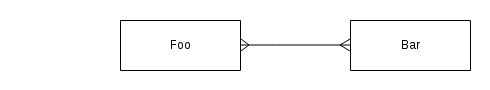
\includegraphics[scale=0.5]{mtm1.png}

\end{frame}

%----------- slide --------------------------------------------------%
\begin{frame}
  \frametitle{Many-to-many}

  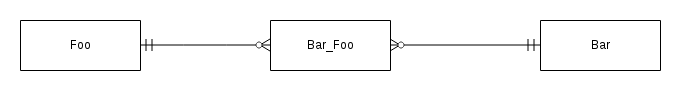
\includegraphics[scale=0.5]{mtm2.png} 

  The \texttt{Bar\_Foo} table holds foreign keys to \texttt{Bar} and 
  \texttt{Foo}.

\end{frame}


%----------- slide --------------------------------------------------%
\begin{frame}
  \frametitle{Intermediate object or not?}

 Do we need an intermediate object or just a join table?
 \begin{itemize}
  \item Use an intermediate object when there is additional data besides
        the joining relationship.
  \item Use a join table without an intermediate object when there is no
        additional data carried with the relationship.
 \end{itemize}
\end{frame}


%----------- slide --------------------------------------------------%
\begin{frame}
  \frametitle{Intermediate object example}
  \begin{figure}
   \centering
   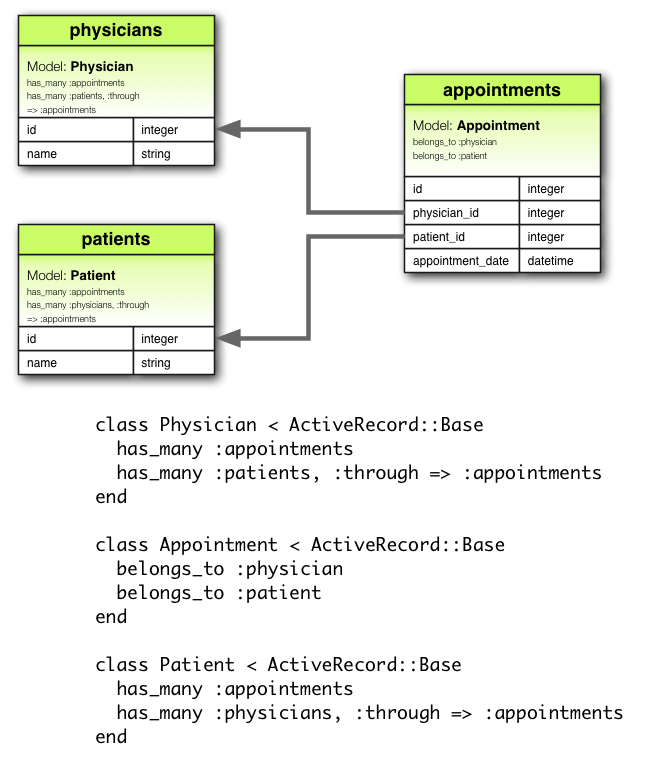
\includegraphics[scale=0.25]{has_many_through.png} \\
   {\scriptsize Source: Rails Guides, \\
   http://guides.rubyonrails.org/association\_basics.html}
  \end{figure}

\end{frame}


%----------- slide --------------------------------------------------%
\begin{frame}[fragile]
  \frametitle{has\_and\_belongs\_to\_many}

 If we only need a join table, we can indicate the many-to-many relationship in the models with \texttt{has\_and\_belongs\_to\_many}.

 \begin{verbatim}
  class Student < ActiveRecord::Base
    has_and_belongs_to_many :classes
  end
 
  class Class < ActiveRecord::Base
    has_and_belongs_to_many :students
  end
 \end{verbatim}

\end{frame}



%----------- slide --------------------------------------------------%
\begin{frame}
  \frametitle{Today's Lab}
 In today's lab, we want to model following, i.e., a user may follow and be followed by other users.  A user who follows another will see the followed user's splatts in her feed.
 \begin{itemize}
  \item We need a self join, \textbf{and}
  \item we need a many-to-many.
 \end{itemize}

This is a little more complicated than the examples we just considered, \emph{but it's still not that hard.}

\end{frame}

\end{document}
